\subsection{\leo{Cycle Complexity Breakdown}}

Given the previous results, we plan to investigate how to improve the
efficiency of the simple V-cycle with 1 relaxation step. The first step is to
breakdown the time spent in the different parts of a cycle. Note that all the
matrices for each level are computed in a setup phase and it is not necessary
to analyze that setup time. We only focus on measuring the following two
computations: (i) the time spent doing a relaxation at each level and (ii) the
time spent computing the next linear system. The later (i.e., computing the
next linear system) can be divided in two options: \emph{going down} by
restricting the solution to a coarser grid, which corresponds to a sparse
matrix-vector computation; and \emph{going up} by interpolating the error term
which also corresponds to another sparse matrix-vector computation.

\begin{table}[htb]
 \resizebox{\linewidth}{!}{
 \begin{tabular}{|c|c|c|c|c|c|c|}
  \hline
  Level & \makecell{Matrix \\ size} & \makecell{Non-zero \\ elements} & \makecell{Relax \\ (down)} & \makecell{Relax \\ (up)} & \makecell{MatVec \\ (down)} & \makecell{MatVec \\ (up)} \\
  \hline
  1 & 512,000 & 4,042,520 & 20 ms & 20 ms & 15 ms & -\\
  \hline
  2 & 256,000 & 6,475,239 & 20 ms & 25 ms & 12 ms & 4 ms\\
  \hline
  3 & 58,893 & 2,000,513 & 8 ms & 8 ms & 3 ms & 2 ms\\
  \hline
  4 & 14,285 & 788,509 & 2 ms & 2 ms & 1 ms & 0.7 ms\\
  \hline
  5 & 4,238 & 386,333 & 1 ms & 1 ms & 0.5 ms & 0.2 ms\\
  \hline
  6 & 609 & 53,493 & 0 ms & 0 ms & 0 ms & 0 ms\\
  \hline
  7 & 69 & 2,873 & 0 ms & 0 ms & 0 ms & 0 ms\\
  \hline
  8 & 2 & 4 & 0 ms & - & - & 0 ms\\
  \hline
 \end{tabular}
 }
 \caption{Time breakdown of a V-cycle with $\alpha=1$.}
 \label{table.measures}
\end{table}

To study the internal time breakdown of a V-cycle we chose as problem an
unstructured domain with some anisotropy (denoted as Unstructured-Anisotropy)
of size 512,000 with a 8-level grid. The results of this evaluations are
depicted in Table~\ref{table.measures}, along with information on the matrix
used at the corresponding level, such as matrix size and the number of non-zero
elements.  Our first observation is that there is a direct correlation between
the time spent on relaxations at each given level and the number of non-zero
entries in the input matrix. Most importantly, in this results we observe that
relaxations represent $\approx66\%$ of the total cost of a V-cycle, while the
matrix-vector multiplications are only $\approx30\%$. In addition, we notice
that the two first levels are the most expensive ones.  It is important to
highlight that in the experiments depicted in Figure~\ref{fig.first_tests},
although different number of relaxations were evaluated, all levels executed
the \emph{same} number of relaxations.

\subsection{\leo{Level-Dependent Relaxation Tuning}}

Based on this information, we propose to reduce the execution time of a V-cycle
by tuning the number of relaxations differently for each level. More precisely
we propose the following two ideas: (i) to add more relaxations in the last
levels because their cost is negligible and they could potentially reduce the
time to convergence or (ii) to remove some relaxations in the first levels to
reduce the computational cost, and see how that affects convergence. We
translate these ideas into the four following strategies (based on a 8-level
grid):

\begin{itemize}
    \item \emph{Fast } : no relaxations at level 2.
    \item \emph{Fast2} : 10 relaxations at level 6.
    \item \emph{Fast3} :  2 relaxations at levels 6 and 4.
    \item \emph{Fast4} : no relaxations at level 3.
\end{itemize}

\begin{figure*}
    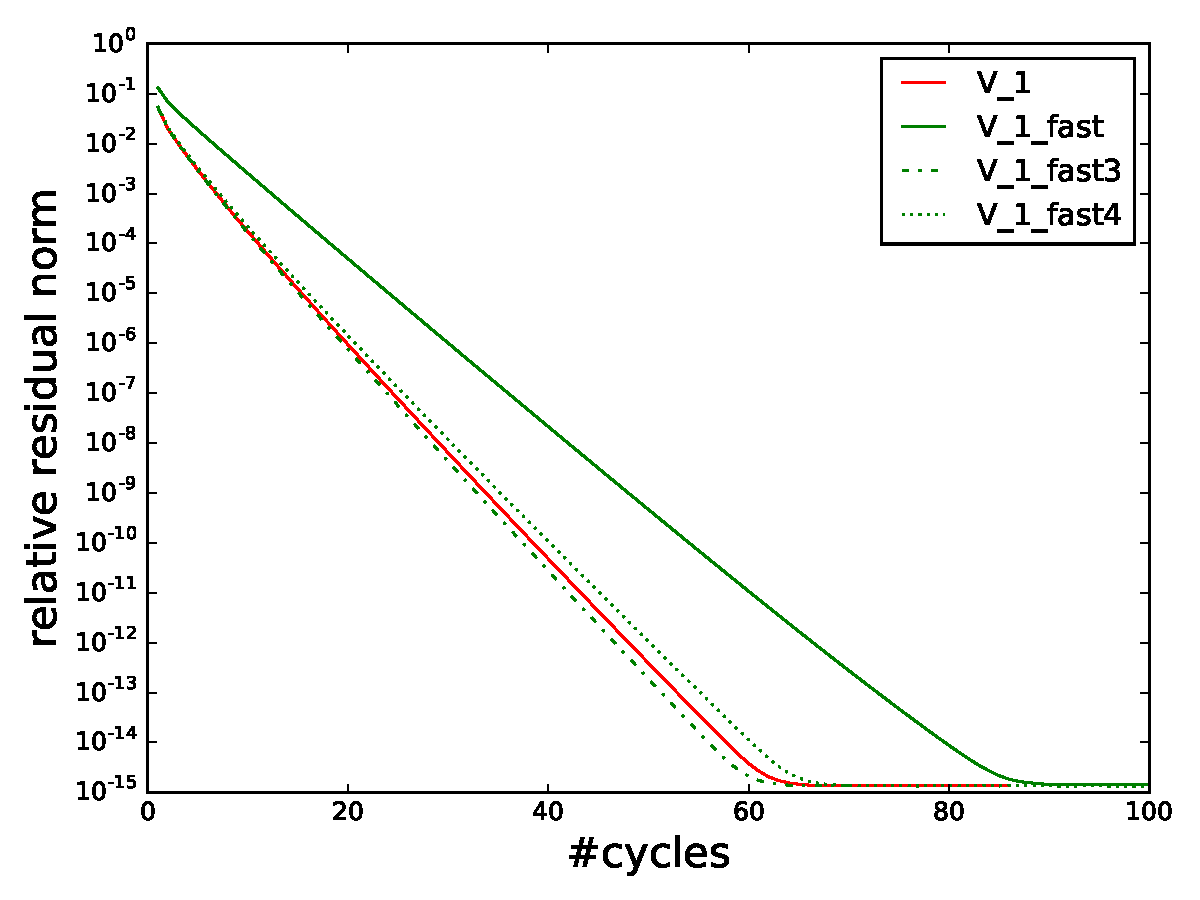
\includegraphics[width=0.33\linewidth]{figs/convergence_fast_norm.pdf}
    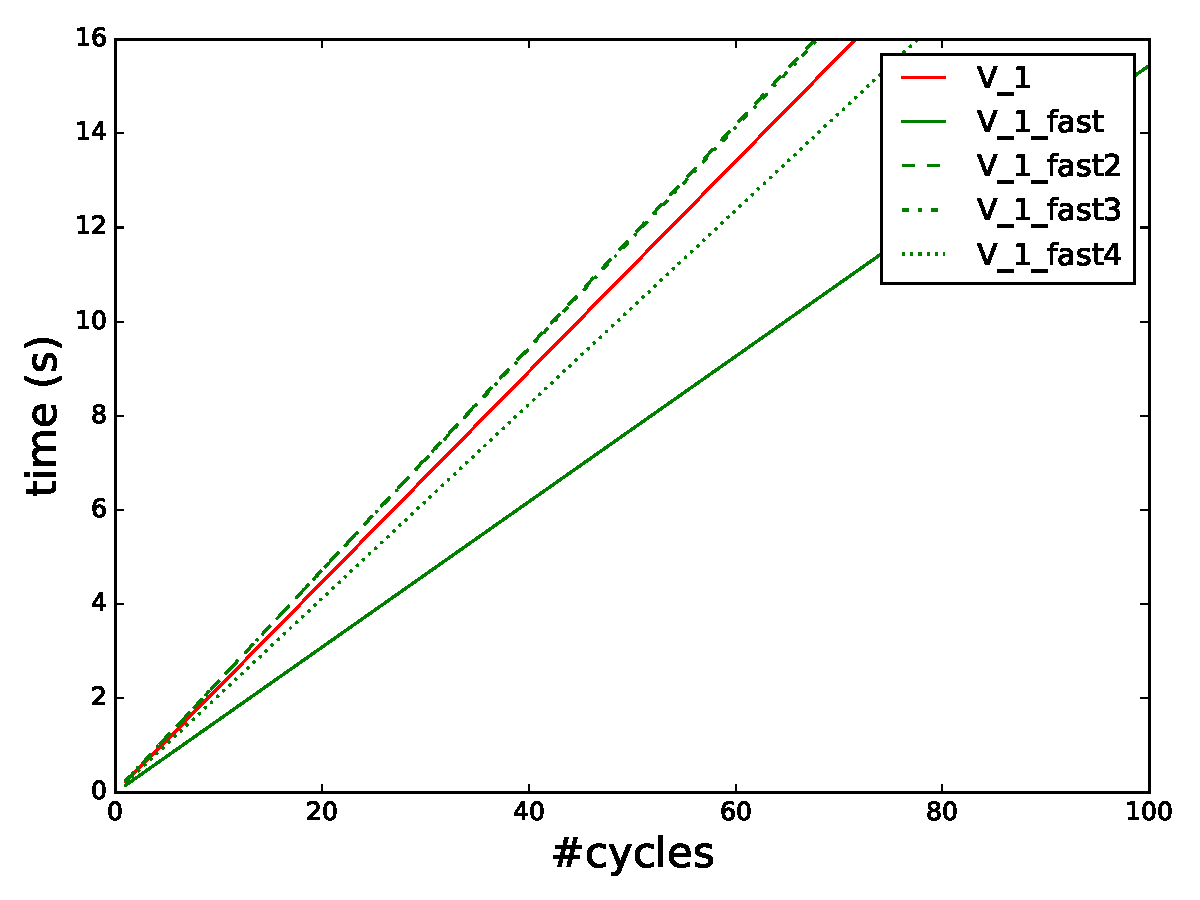
\includegraphics[width=0.33\linewidth]{figs/convergence_fast_time.pdf}
    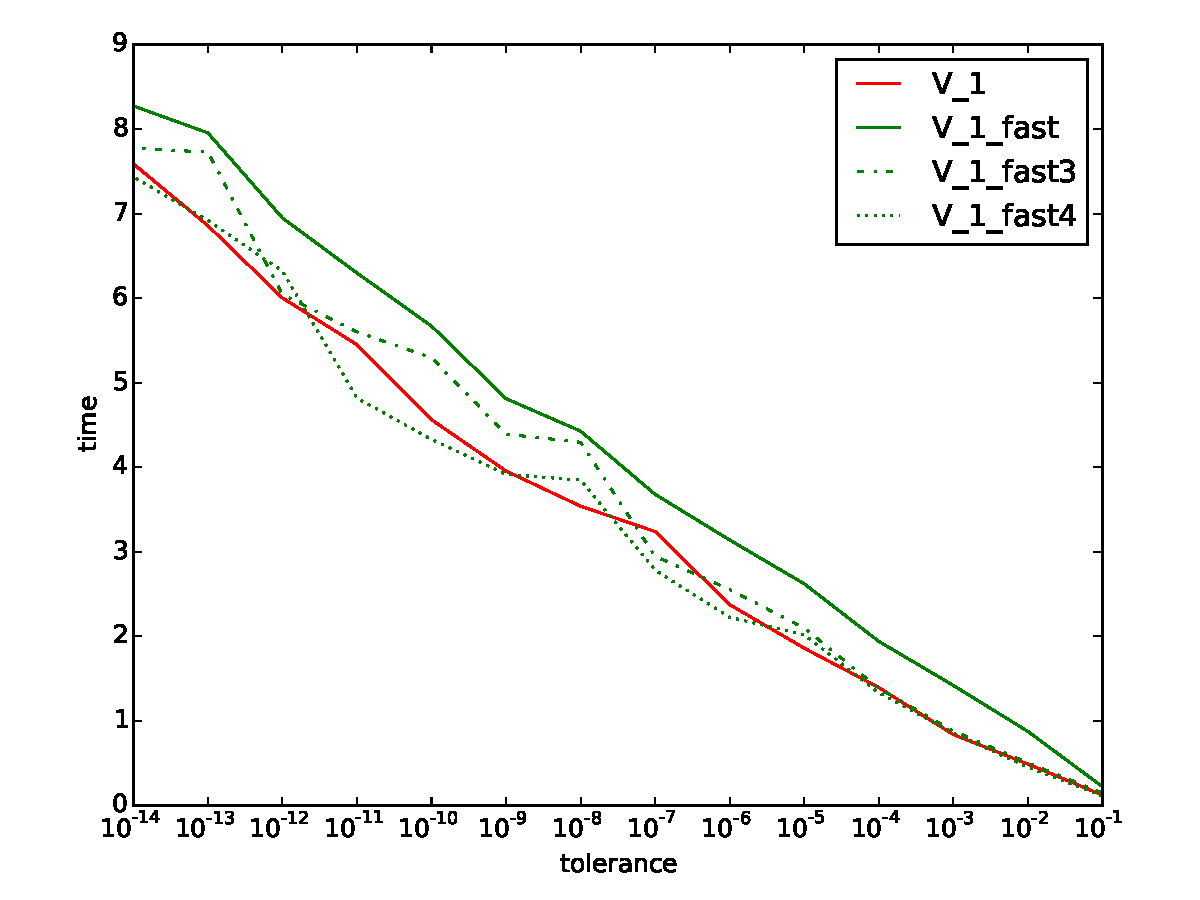
\includegraphics[width=0.33\linewidth]{figs/time_convergence_fast.pdf}
    \caption{Evaluation of 4 level-dependent relaxation tuning strategies.
    Residual norm per cycle (left), time spent in each cycle (middle) and
    convergence time in function of the error tolerance (right).}
    \label{fig.newstrat}
\end{figure*}

The strategy \emph{Fast} aims at reducing the cost of the cycle by removing the
penultimate relaxation which is very expensive, and expecting that the accuracy
lost at this point can be compensated by the relaxation at level 1.  The
strategy \emph{Fast2} executes a lot of relaxations at level 6, because it
should not increase by much the execution time of the V-cycle.  The reason to
choose level 6 instead of level 7 or 8 is that the relaxation at level 8 is
actually a direct solve. Thus, the result term is almost exact at level 7,
because the only source of error comes from the interpolation of $e^8$ (which
is exact) into $e^7$. This is why, we might expect better results by adding
relaxations at level 6. The strategy \emph{Fast3}, pushes the previous idea one
step further. If we assume that doing more than one relaxation gets a more
accurate error estimation at level $l$, then at level $l-1$ we do not need to
correct a lot by doing more relaxations. However at level $l-2$ we have been
through 2 interpolations since the last good estimation of the error vector,
therefore we increasing the number of relaxations again. Since the first levels
are very expensive, we stop this recursion at level 3.  Finally, we propose one
last strategy \emph{Fast4} which is a softer version of \emph{Fast} where the
relaxation at level 3 is removed, producing a less accurate result at that
point, but expecting it can be compensated by the two relaxations at level 1
and 2.

%\begin{figure*}
%    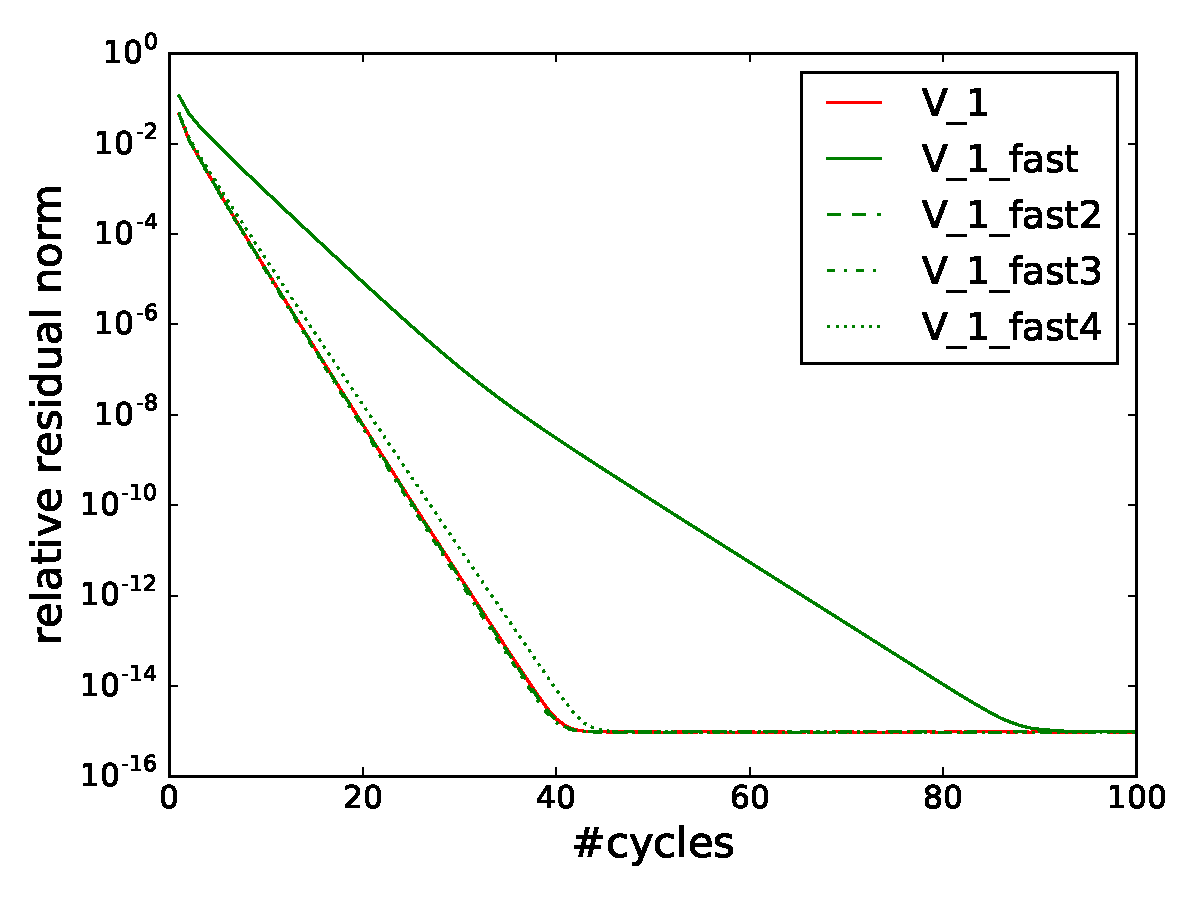
\includegraphics[width=0.33\linewidth]{figs/convergence_fast_small_norm.pdf}
%    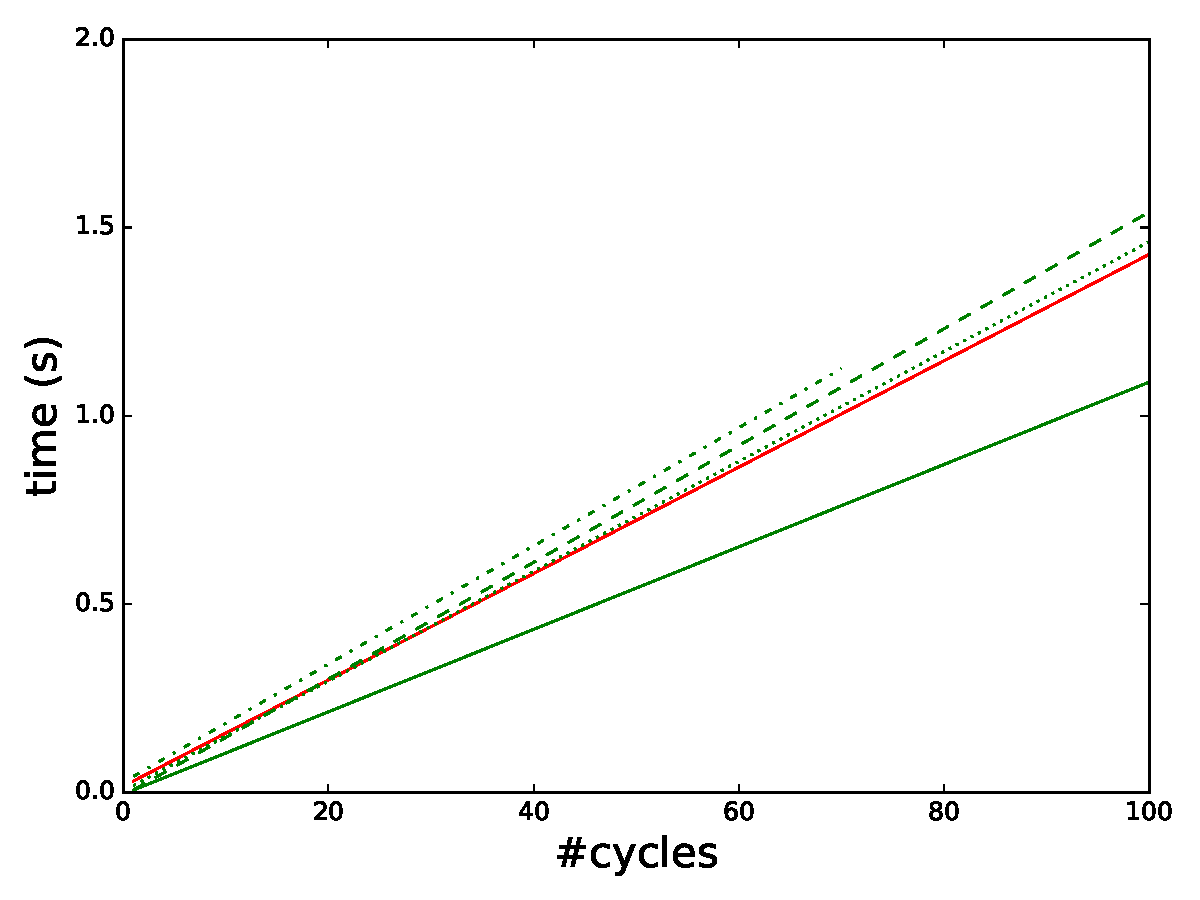
\includegraphics[width=0.33\linewidth]{figs/convergence_fast_small_time.pdf}
%    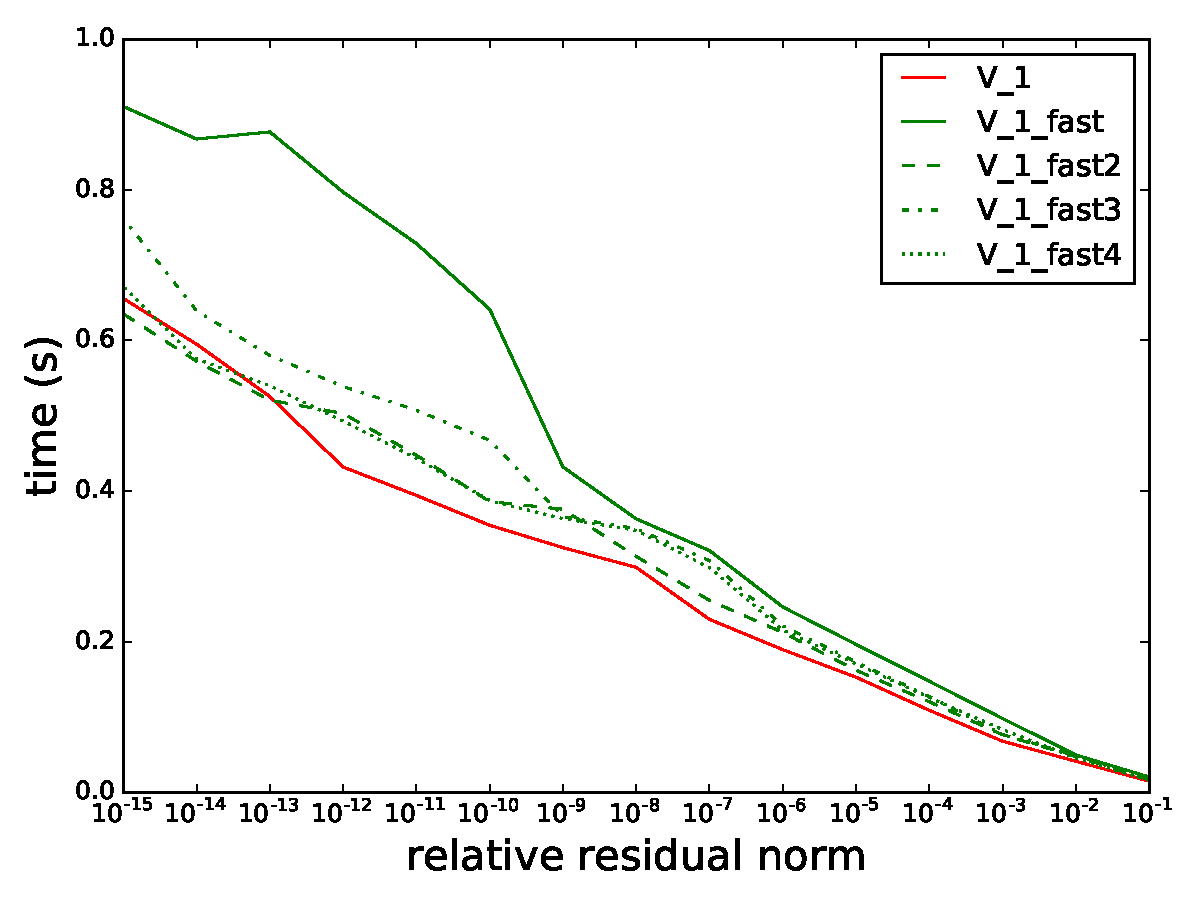
\includegraphics[width=0.33\linewidth]{figs/time_convergence_fast_small.pdf}
%    \caption{Final residual norm of the 4 new strategies per iteration (left),
%    interpolated execution time per iteration (middle) and convergence time as
%    a function of the tolerance (right) on a small matrix.}
%    \label{fig.newstrat_small}
%\end{figure*}

We evaluated these 4 proposed strategies in the original $512,000\times
512,000$ matrix.  The results are shown in Figure~\ref{fig.newstrat}.  The
first thing to observe is that removing the relaxation at level 1 does not
provide any benefit. It does saves time during each cycle but the accuracy loss
too high in each cycle, leading to a much slower convergence rate (i.e., more
cylces needed for convergence).  The other thing to notice is that adding more
relaxations in the last levels slightly increases the execution time but it
does not provide any benefit on the accuracy side. Thus, strategies
\emph{Fast2} and \emph{Fast3} are not really efficient.  Only the strategy
\emph{Fast4} seems to be more or less equivalent to the original V cycle as it
reduces a bit the cost of each cycle and the convergence rate per cycle is also
slightly smaller.  More tests were performed on a smaller matrix with an
initial matrix size of 64,000 with only a 6-level grid.  The results were
similar and are not shown in this paper for brevity.


%We find again that the original V cycle seems to be the best as \emph{Fast3}
%converges in slightly less cycles, but this strategy is clearly too expensive
%with a bigger matrix so overall it is not as efficient as the baseline.


\subsubsection{An asymmetric strategy}
\label{sec.assymetric}
  We observe no big improvement compared to the original V-cycle with 1 relaxation at each level with the previous strategies.
  Their common point is that they all do the same number of relaxations when going down or up in the cycle. However, the main idea of the multi-grid algorithm is totally asymmetric: the relaxations before
going to a coarser level is there to compute a first approximate solution to the current system while the relaxations before going back to a finer level are here to refine the error term.
  We first compute an approximation at a given level $l$, then we use the level $l+1$ to compute an approximate error term $e^l$ and finally we redo some relaxation to refine the solution. The two relaxations do not have the same goal.
  What if we could ensure that any value of the error vectors will be less than $\epsilon$ from the exact value just by doing a relaxation step? We would not need to do a relaxation
  before computing the approximate error term using the next levels in the grid but compute directly the error term when we go back up in the cycle. From that idea we define a new asymmetric strategy: we use a V-cycle with $\alpha_1 = 0$ and $\alpha_2 = 1$. In other words
  we do one relaxation at each level only when we are going up in the cycle. We call this strategy \emph{Up}.

  We run \emph{Up} and \emph{Fast4}, as long as the classical V-cycle, on the same matrix of size 512,000 and also on
  other applications (3D laplace with a 9-pt stencil, 3D laplace with a 27-point stencil, and another 3D partial derivative equation with Dirichlet boundary conditions) with the same size of matrix.

  All results are presented in Figure~\ref{fig.up_comparison}.

  \begin{figure*}
    \centering
   \subfloat[\textsc{Unstructured-Anisotropy}]{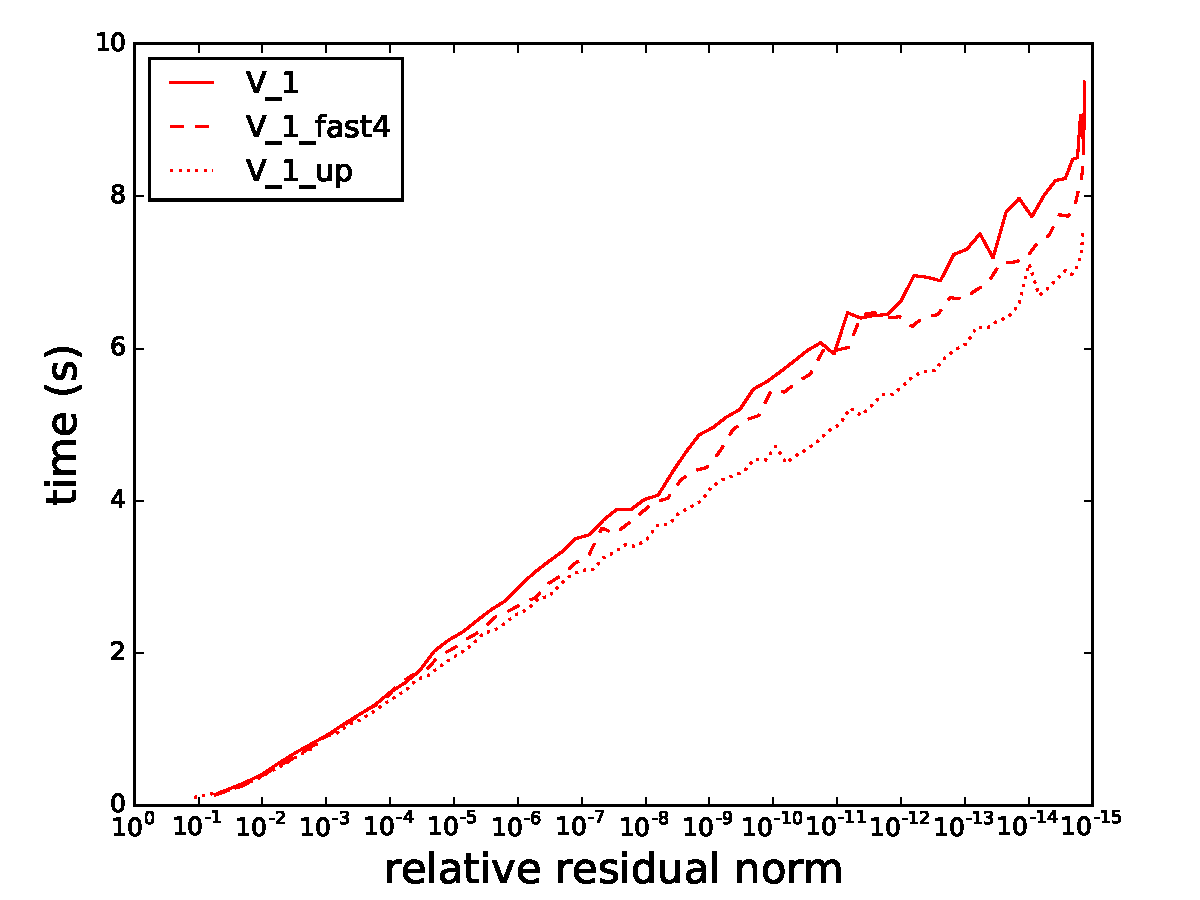
\includegraphics[width=0.4\linewidth]{figs/time_convergence_up_1.pdf}}
   \subfloat[\textsc{3DLaplace-9pt}]{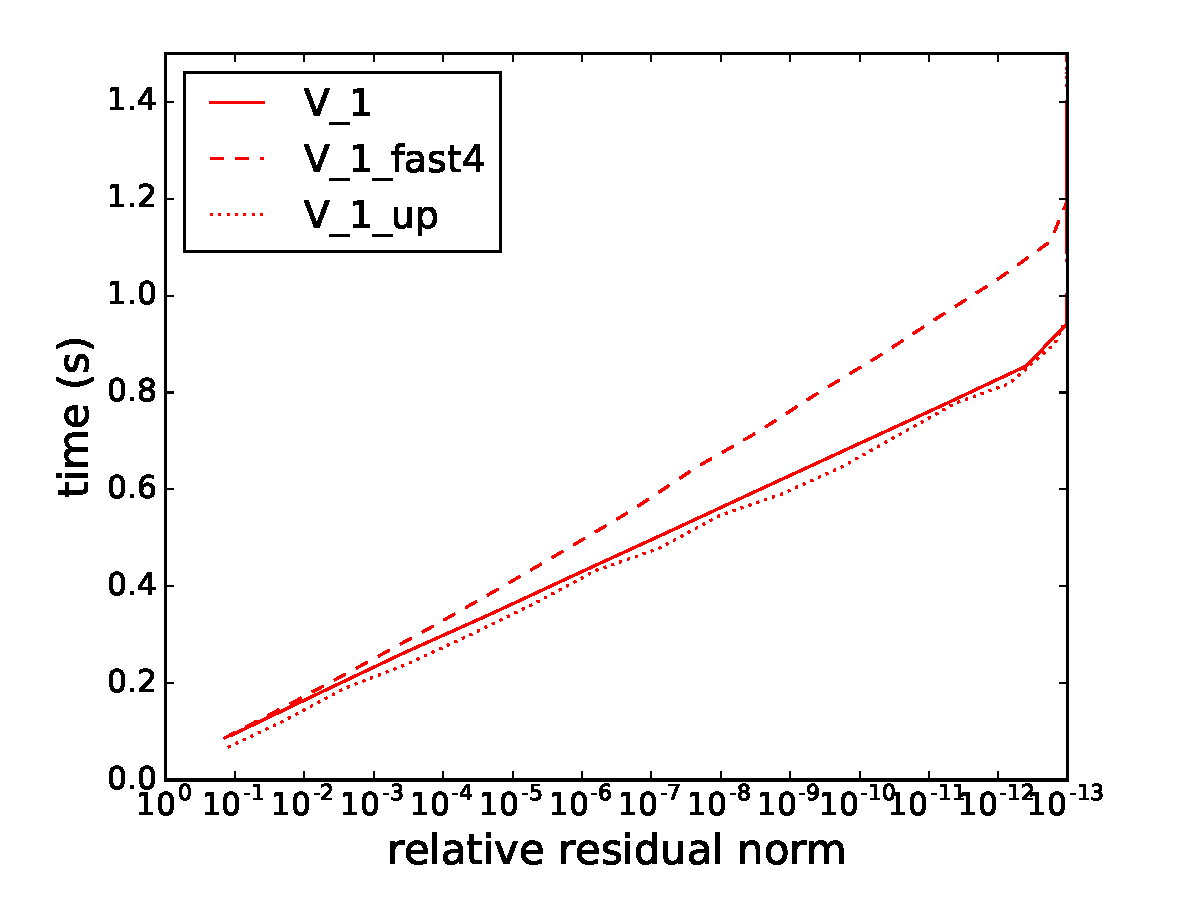
\includegraphics[width=0.4\linewidth]{figs/time_convergence_up_2.pdf}}\\
   \subfloat[\textsc{3DLaplace-27pt}]{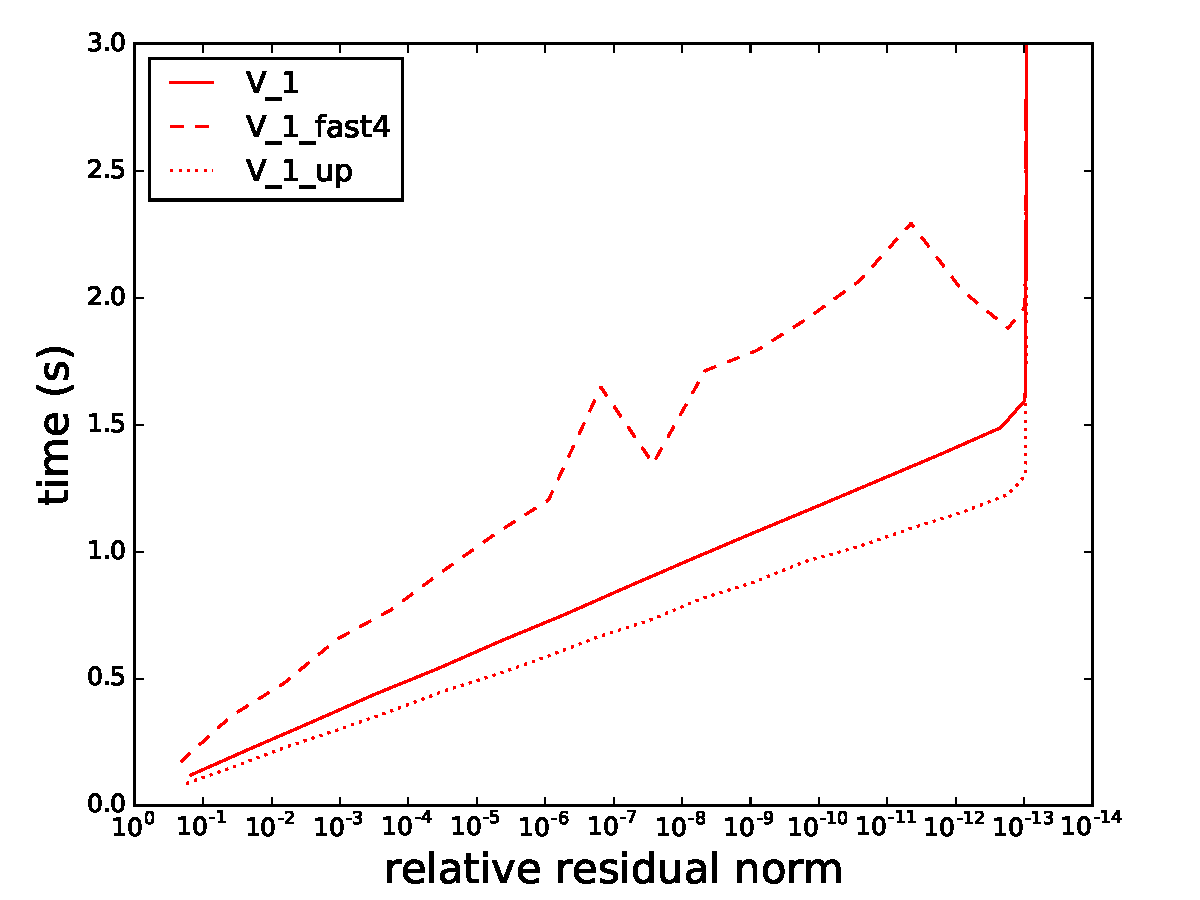
\includegraphics[width=0.4\linewidth]{figs/time_convergence_up_3.pdf}}
   \subfloat[\textsc{PDE-Dirichlet}]{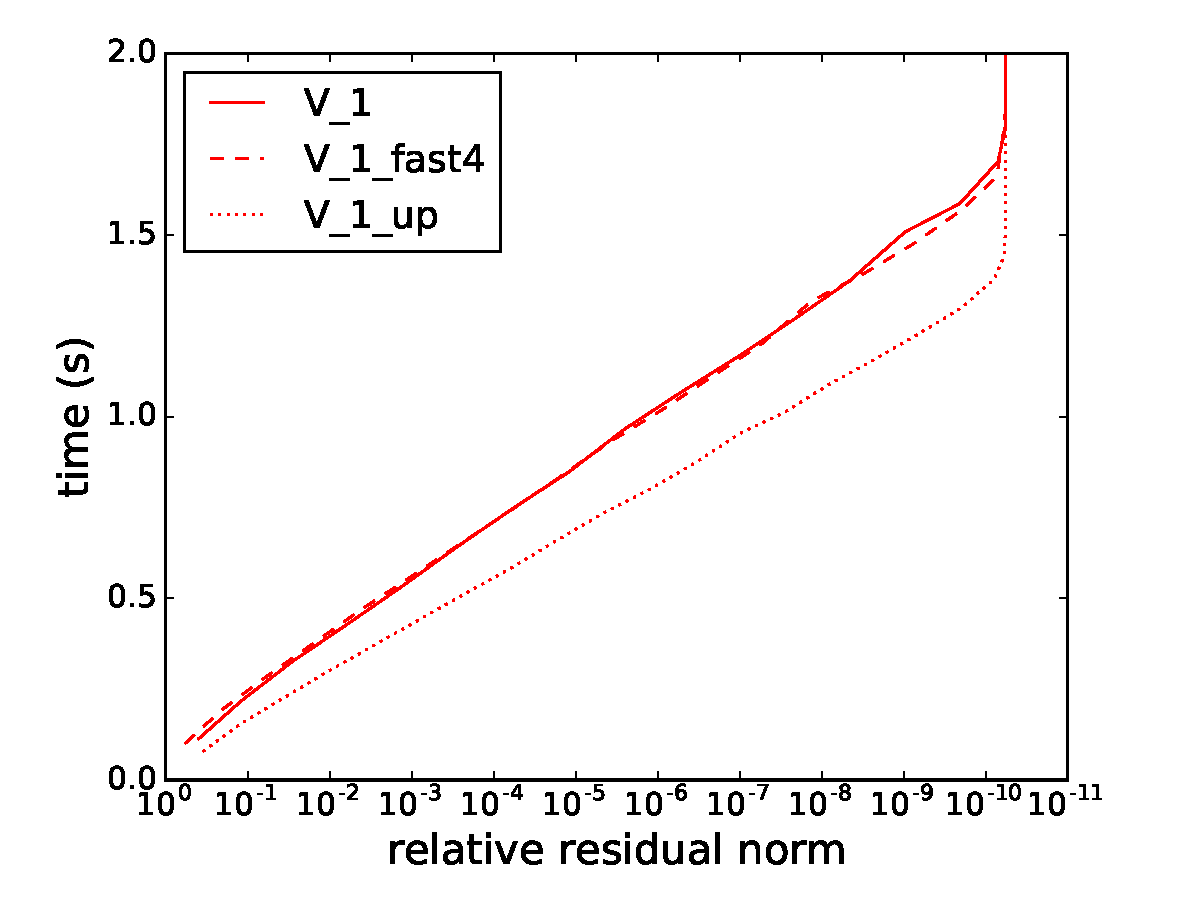
\includegraphics[width=0.4\linewidth]{figs/time_convergence_up_4.pdf}}
   \caption{Comparison of original algorithm with \emph{Fast4} and \emph{Up} strategies.}
   \label{fig.up_comparison}
  \end{figure*}

   At this point, we see that it is not worth considering the \emph{Fast4} strategy anymore. However, \emph{Up} seems to be
   quite efficient since it improves by $12\%$,$7\%$,$20\%$ and $22\%$ (for \textsc{Unstructured-Anisotropy}, \textsc{3DLaplace-9pt}, \textsc{3DLaplace-27pt} and \textsc{PDE-Dirichlet} respectively) the average time needed to reach
   a $10^{-i}$ precision.
   However all these runs are sequential and does not guarantee the viability of the \emph{Up} strategy when the algorithm is parallelized.
   More tests were performed on MinoTauro with bigger matrices and different processor topologies. The total size of the matrix is set to either
   5,832,000 or 13,824,000, while the topology will be composed of either 27 (3x3x3), 36 (6x6x1) or 64 (4x4x4) processors, where each processor holds 1 MPI process and there is only 1 OpenMP thread per process.
   The problems tested were \textsc{3DLaplace-9pt} and \textsc{3DLaplace-27pt}.
   For these 6 possible combinations, we observe an averaged improvement of 18.4\% (ranging from 16.0\% to 28.3\%) for \textsc{3DLaplace-9pt} and 20.5\% (ranging from 16.2\% to 25.0\%) for \textsc{3DLaplace-27pt}. It seems that \emph{Up} outperforms
   even more the classical V-cycle when the problem size increases, but seems to cap at around 25\% improvement. Figure~\ref{fig.mtup} presents the results for the matrix size 13,824,000 and \textsc{3DLaplace-27pt}, for the 3 different processor topologies. We have similar figures
   for the other scenarios.

   \begin{figure*}[t]
    \subfloat[3x3x3]{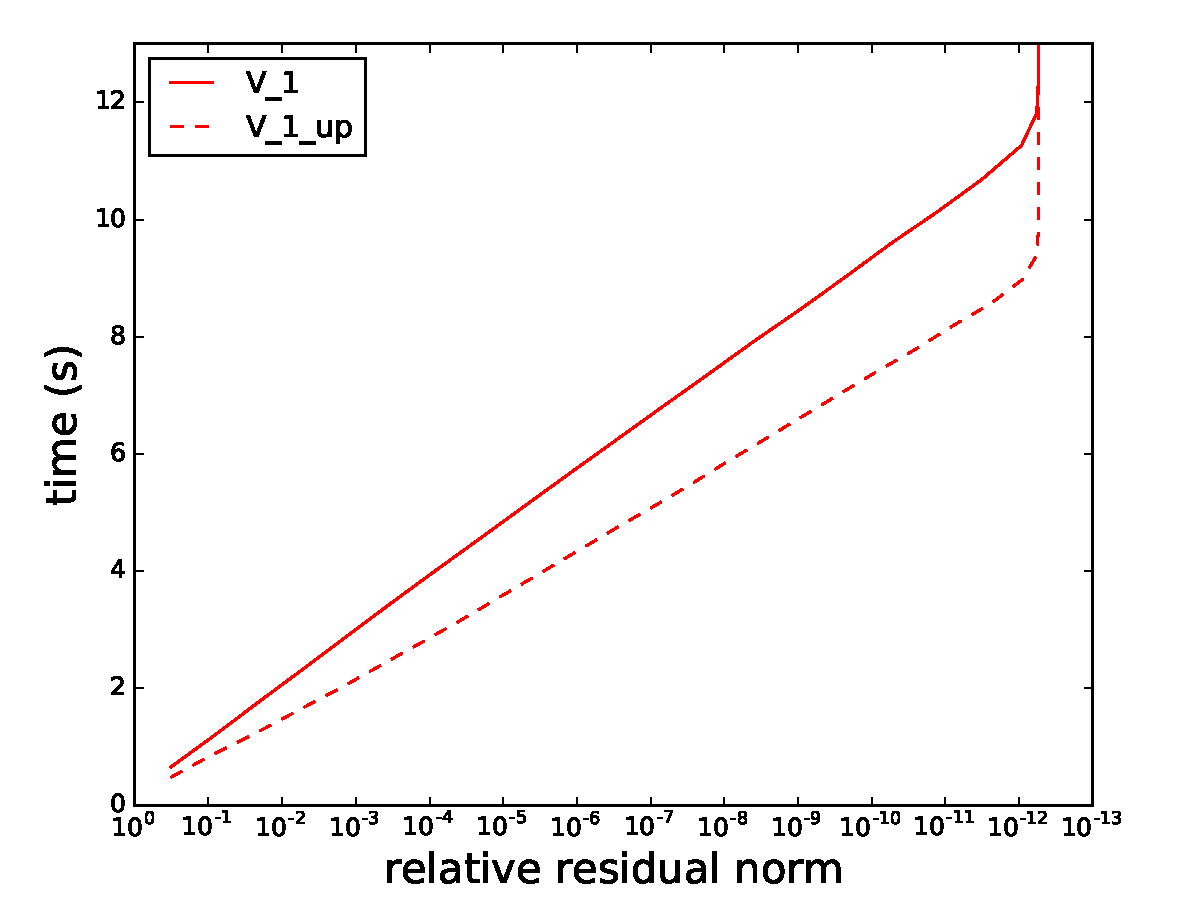
\includegraphics[width=0.33\linewidth]{figs/mt_27.pdf}}
    \subfloat[4x4x4]{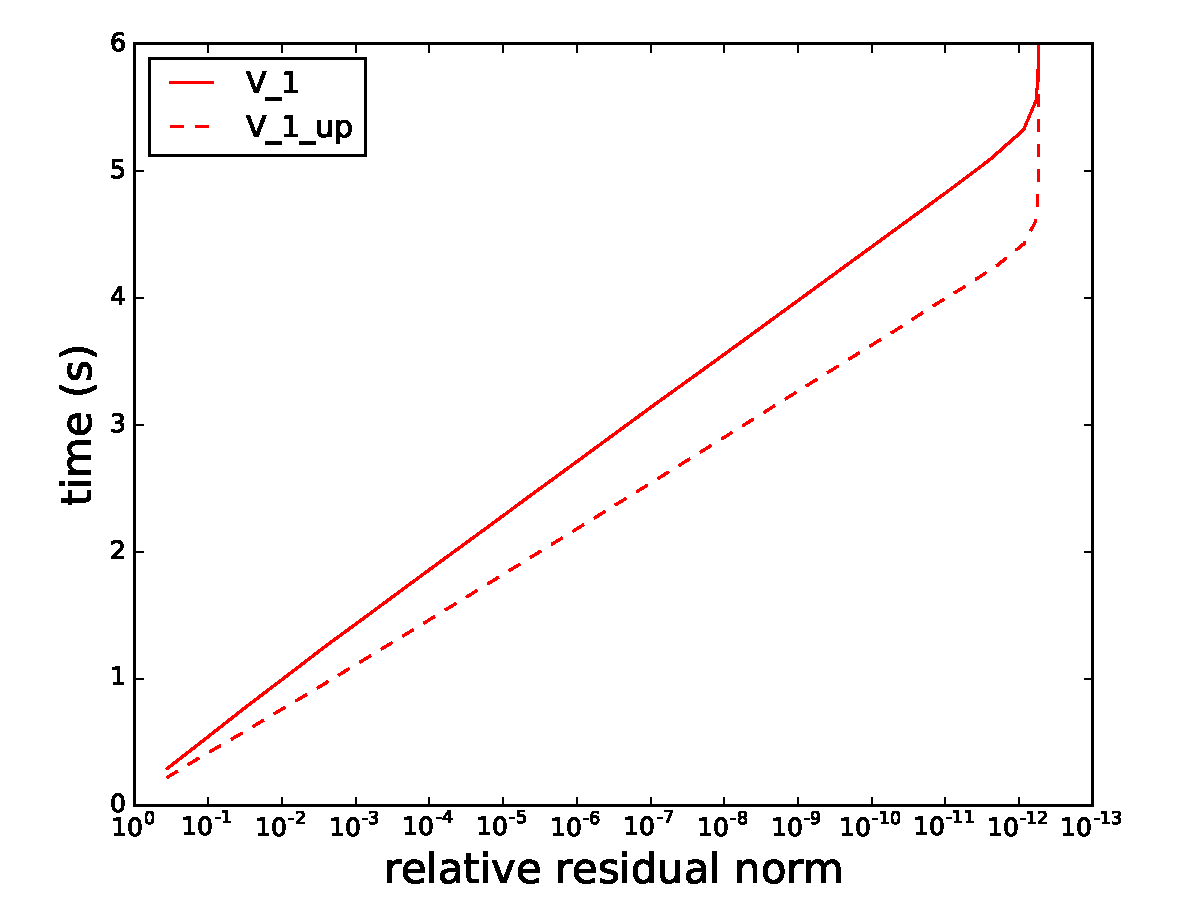
\includegraphics[width=0.33\linewidth]{figs/mt_64.pdf}}
    \subfloat[6x6x1]{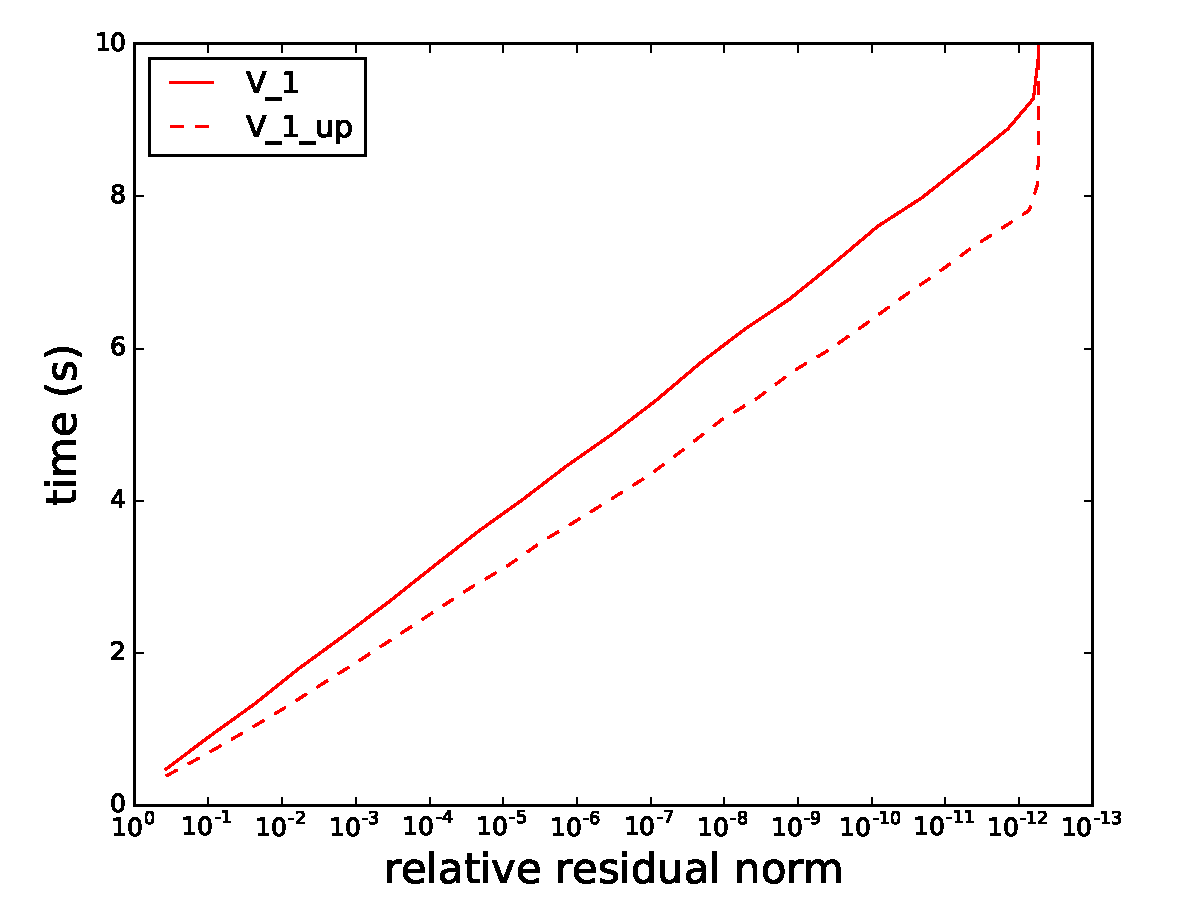
\includegraphics[width=0.33\linewidth]{figs/mt_36.pdf}}
    \caption{Comparison of original algorithm with \emph{Up} strategy for \textsc{3DLaplace-27pt} on a 240x240x240 grid.}
    \label{fig.mtup}
   \end{figure*}
